\chapter{Applying Greedy PRM to Multi-Set: the Multi-Set Greedy PRM}
\label{chap:multi-set-prm}

\begin{itemize}
\item GreedyPRM and multi-set are complementary
\item Apply greeydprm to multi-set problem
\item one planner that learns, can answer arbitrary queries
   in multiple related spaces faster and faster
\end{itemize}

\section{From RSS Intro}

This computational burden is especially troublesome
in time-sensitive human-scale manipulation tasks
(e.g. from household or disaster response domains).
The costs incurred by the planner
(computation time / electrical energy)
and the robot's motor controllers
(execution time / mechanical energy)
tend to be of comparable magnitude in such domains.
As a result,
we'd like an approach which can reason about both
planning \emph{and} execution costs,
striving for a balance between feasibility and optimality.

Our second key insight
is to apply the principle of best-first search over roadmaps
using an objective which explicitly considers both planning and
execution costs.
The result is the Multi-Set PRM (Section~\ref{chap:multi-set-prm}).
This approach allows the planner to exploit the multi-set structure
inherent in these problems.
%We show the relation of this approach to inflated heuristics
%when applied to traditional graph search over implicit graphs.

\section{Related Work}

Also, there are incremental E-graphs \cite{phillips2013anytimeegraphs}
that we should relate the planner to and compare with.

\section{Implementation Details}

\subsection{Calculating the Optimistic Path Cost}
\label{subsec:alg-opt-path-cost}

The execution cost component is given by $f_e[x(t)]$
as defined in the cost model $\mathcal{M}$
(Section~\ref{subsec:cost-model}).
The optimistic estimate of the remaining planning cost for the path
is computed by determining the cost of the optimistic plan for each
edge using the \textsc{OptEdgePlan} function
(Section~\ref{subsec:alg-opt-edge-plan}).

\begin{algorithm}
\caption{Calculating the Optimistic Edge Plan}
\label{alg:opt-edge-plan}
\begin{algorithmic}[1]
\Function {$\mbox{\textsc{OptEdgePlan}}$}{$e$}
   \State $(S_{best}, b_{best}, c_{best})
      \leftarrow (\mbox{\textbf{nil}}, \mbox{\textbf{nil}}, \infty)$
   \ForAll {$S \in \mathcal{P}(\mathcal{S})$}
         \label{line:power-set}
      \State $c = \sum_{X \in S} f_X[e]$
      \ForAll {$b \mbox{ \textbf{s.t.} }
            b : S \rightarrow \{\mbox{True},\mbox{False}\}$}
            \label{line:all-binary-functions}
         \State $\arraycolsep=2pt
            P_{new} =
            \left\{\left.\left( \begin{array}{rl}
            \mathbf{1}_X & \mbox{if } b(X) \\
            \lnot \mathbf{1}_X & \mbox{otherwise} \\
            \end{array} \right)
            \right|
            X \in S
            \right\}$
         \If {$P_{rels} \cup e.P \cup P_{new}
               \Rightarrow \mathbf{1}_{X_g}$ is valid}
            \If {$c < c_{best}$}
               \State $(S_{best}, b_{best}, c_{best})
                  \leftarrow (S, b, c)$
            \EndIf
         \EndIf
      \EndFor
   \EndFor
   \State \Return $(S_{best}, b_{best}, c_{best})$
\EndFunction
\end{algorithmic}
\end{algorithm}

\subsection{Calculating the Optimistic Edge Plan}
\label{subsec:alg-opt-edge-plan}

The \textsc{OptEdgePlan} function (Alg.~\ref{alg:opt-edge-plan})
performs the core reasoning which exploits the relations in
the multi-set problem.
Before discussing its implementation,
we first briefly discuss the propositional logic approach
used to reason about the state of each edge.

The planner represents the list of set relations $\mathcal{R}$
(Section~\ref{subsec:problem-definition})
specified in the multi-set problem formulation
as a set of \emph{logical propositions} $P_{rels}$
which are considered globally applicable.
For example,
the proposition $\mathbf{1}_A \Rightarrow \mathbf{1}_B$
follows from the relation $A \subseteq B$
(see Fig.~\ref{fig:relations}).
In addition,
each edge $e$ in the roadmap is augmented with an initially empty
set $e.P$ containing all additional edge-specific propositions
known to be true as a result of any indicator functions evaluated
over that edge.
For example,
if planner evaluated the indicator $\mathbf{1}_B[e]$
and it returned False,
the proposition $\lnot\mathbf{1}_B$ would be added to $e.P$.
Together, such sets of propositions can be used as \emph{premises}
as part of an \emph{argument} to demonstrate a \emph{conclusion};
a logical solver can then be used validate or invalidate the argument.
For example, an argument with these premises and conclusion
$\{ (\mathbf{1}_A \Rightarrow \mathbf{1}_B), (\lnot\mathbf{1}_B) \}
\Rightarrow (\lnot\mathbf{1}_A)$
can be shown to be valid.

The \textsc{OptEdgePlan} function (Alg.~\ref{alg:opt-edge-plan})
is tasked with computing
the optimistically optimal set of indicator evaluations to perform
for the edge in order to validate its membership in the query
$\mathcal{C}$-subset $X_g$.
The function returns three elements:
(a) the set of $\mathcal{C}$-subsets $S \subseteq \mathcal{S}$
whose indicators are to be evaluated,
(b) a binary function $b$
which provides the desired indicator result for each evaluation,
and (c) the total evaluation cost $c$
given by the cost model $\mathcal{M}$'s $f_X[\cdot]$ functionals
(Section~\ref{subsec:cost-model}).

The function proceeds by considering all combinations of
available $\mathcal{C}$-subset indicators $S$ (line~\ref{line:power-set}).
For each set of evaluations,
we compute the planning cost $c$ which would be required.
We then consider all possible outcomes for each indicator
by iterating over all functions $b$ mapping
from $\mathcal{C}$-subset $X$ to binary values
(line~\ref{line:all-binary-functions}).
For each potential outcome $b$,
we form the set of additional propositions $P_{new}$,
and then use a logic solver to determine whether the aggregate
premises imply membership in the query $\mathcal{C}$-subset $X_g$.
If so (and the required cost is the best so far),
we save and return it.

\subsection{Home Robot Manipulation Task}
\label{subsec:herb-experiment}

\begin{figure*}
\begin{widepage}
\centering

\begin{subfigure}[t]{0.185\linewidth}
\centering
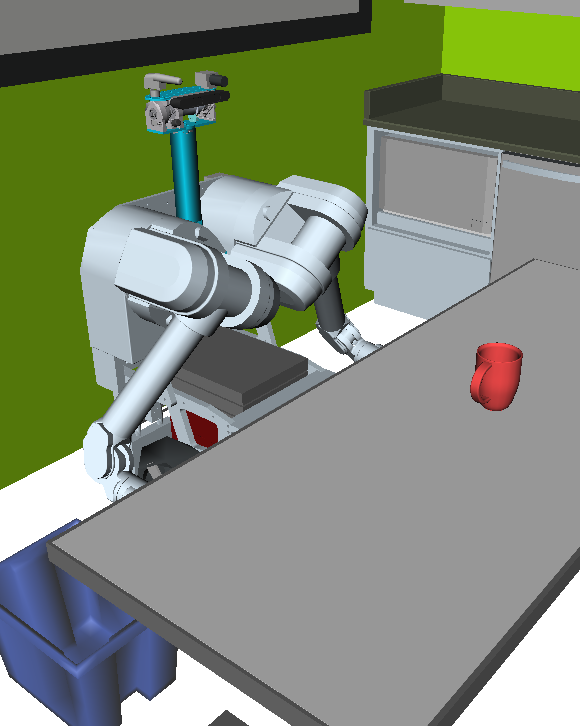
\includegraphics[width=\columnwidth]{figs/testherb-a.png}
\caption{Starting Configuration}
\end{subfigure}
\begin{subfigure}[t]{0.185\linewidth}
\centering
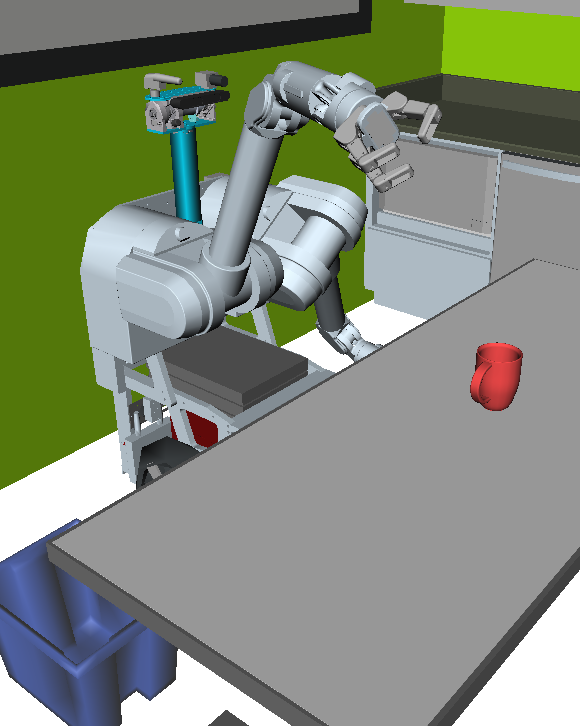
\includegraphics[width=\columnwidth]{figs/testherb-b.png}
\caption{Step 1, in $X_1$}
\end{subfigure}
\begin{subfigure}[t]{0.185\linewidth}
\centering
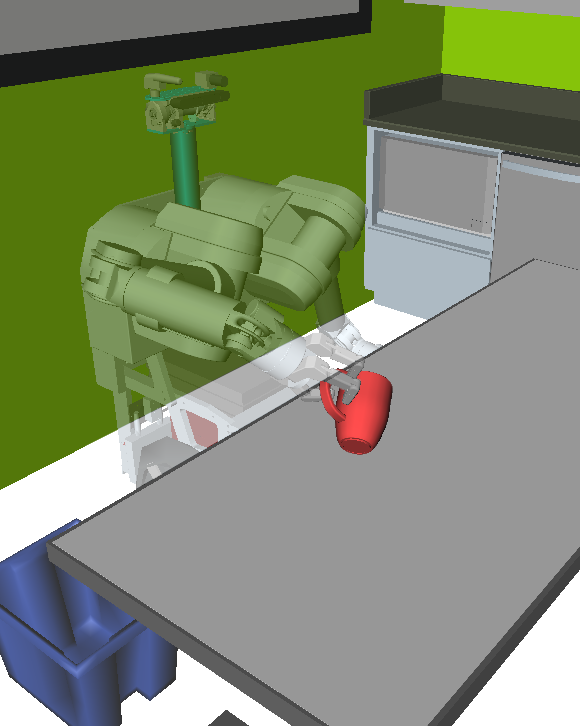
\includegraphics[width=\columnwidth]{figs/testherb-c.png}
\caption{Step 2, in $X_2$}
\end{subfigure}
\begin{subfigure}[t]{0.185\linewidth}
\centering
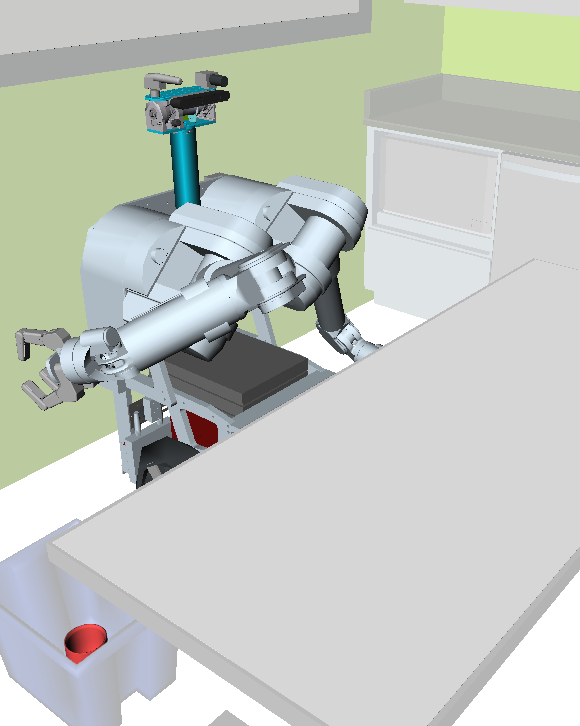
\includegraphics[width=\columnwidth]{figs/testherb-d.png}
\caption{Step 3, in $X_3$}
\end{subfigure}
\begin{subfigure}[t]{0.185\linewidth}
\centering
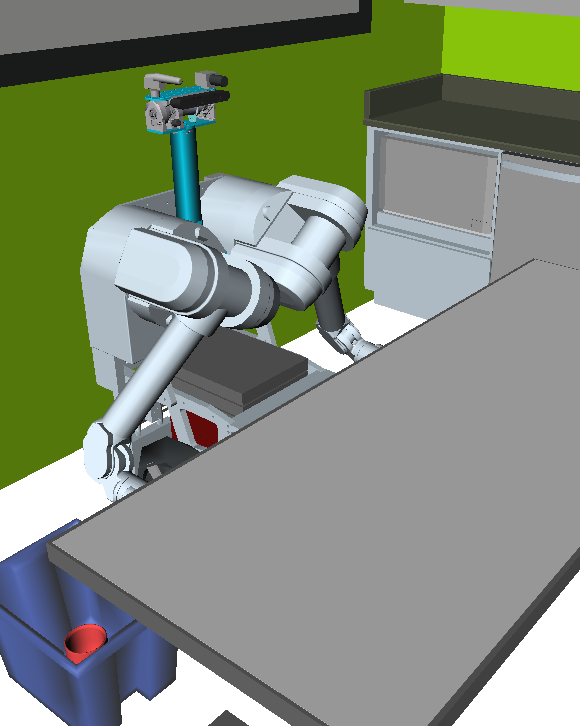
\includegraphics[width=\columnwidth]{figs/testherb-e.png}
\caption{Ending Configuration.}
\end{subfigure}

\caption{
  A home robot performing a three-step manipulation task.
  It must move from its home configuration
  to grasp the cup,
  transfer it to a drop location above the bin,
  and return home.
  Experimental results for the Multi-Set PRM
  are shown in Table~\ref{tab:testherb}}
\label{fig:testherb-problem}
\end{widepage}
\end{figure*}

\begin{table*}
\begin{widepage}
\centering
\footnotesize
\setlength{\tabcolsep}{3pt}
\renewcommand{\arraystretch}{1.3}
\begin{tabular}{|cc|r@{ }lr@{ }lr@{ }lr@{ }l|r@{ }lr@{ }lr@{ }lr@{ }l|r@{ }lr@{ }lr@{ }lr@{ }l|}
\toprule
\multirow{2}{*}{Relations} & \multirow{2}{*}{Cost}
  & \multicolumn{8}{c|}{$\lambda = 0$}
  & \multicolumn{8}{c|}{$\lambda = 0.5$}
  & \multicolumn{8}{c|}{$\lambda = 1$}
\\
  &
  & Step & 1 & Step & 2 & Step & 3 & \multicolumn{2}{c|}{Total}
  & Step & 1 & Step & 2 & Step & 3 & \multicolumn{2}{c|}{Total}
  & Step & 1 & Step & 2 & Step & 3 & \multicolumn{2}{c|}{Total}
\\ \midrule
\multirow{2}{*}{None} & Plan
  &  6.16&s &  3.72&s &  2.38&s & 12.25&s
  &  5.52&s &  2.89&s &  2.12&s & 10.53&s
  &  3.39&s &  2.25&s &  2.12&s &  7.76&s
\\
  & Exec
  & 14.22&rad &  8.51&rad &  4.23&rad & 26.97&rad
  & 15.07&rad & 10.60&rad &  4.23&rad & 29.89&rad
  & 15.07&rad & 10.60&rad &  4.23&rad & 29.89&rad
\\ [1ex]
Inter-Step & Plan
  &  6.40&s &  2.33&s &  0.86&s &  9.59&s
  &  5.40&s &  1.55&s &  0.91&s &  7.86&s
  &  3.38&s &  0.91&s &  0.30&s &  4.59&s
\\
(Sec.~\ref{subsec:dynamic-environments},~\ref{subsec:grasped-objects})
  & Exec
  & 14.22&rad &  8.51&rad &  4.23&rad & 26.97&rad
  & 15.07&rad & 12.21&rad &  4.23&rad & 31.51&rad
  & 15.07&rad & 12.21&rad &  7.11&rad & 34.40&rad
\\ [1ex]
Self-Checked & Plan*
  &  3.54&s &  2.23&s &  1.17&s & 6.94&s
  &  2.99&s &  1.77&s &  1.16&s & 5.92&s
  &  1.47&s &  1.22&s &  1.16&s & 3.85&s
\\
(Sec.~\ref{subsec:cached-self-valid}) & Exec
  & 14.22&rad &  8.51&rad &  4.23&rad & 26.96&rad
  & 14.22&rad & 10.06&rad &  4.23&rad & 28.51&rad
  & 14.22&rad & 10.60&rad &  4.23&rad & 29.05&rad
\\ [1ex]
\multirow{2}{*}{Both} & Plan*
  &  3.25&s &  1.79&s &  0.90&s & 5.94&s
  &  2.88&s &  1.55&s &  0.92&s & 5.35&s
  &  1.47&s &  1.88&s &  0.31&s & 3.66&s
\\
  & Exec
  & 14.22&rad &  8.51&rad &  4.23&rad & 26.96&rad
  & 14.22&rad &  8.51&rad &  4.23&rad & 26.96&rad
  & 14.22&rad &  9.64&rad &  6.36&rad & 30.22&rad
\\ 
\bottomrule
\end{tabular}
\caption{Home robot manipulation task results.
  The entry with no relations and $\lambda=0$ is equivalent
  to the LazyPRM.}
\label{tab:testherb}
\end{widepage}
\end{table*}

We tested the Multi-Set PRM on the manipulation task
described in Fig.~\ref{fig:testherb-problem}.
We used the $r$-disk PRM construction rule with $r=2.0$ rad,
and a batch size of $N=1000$.
Planning times are measured on a Lenovo T430 laptop.
The planner was asked to solve each of the steps of the plan
sequentially.

We varied
(a) the planning vs. execution parameter $\lambda$
(see Section~\ref{subsec:alg-opt-path-cost}), and
(b) the subset relations provided to the planner
as described in Sections
\ref{subsec:dynamic-environments},
\ref{subsec:grasped-objects},
and \ref{subsec:cached-self-valid}.
We measured the time required for planning (s)
and the length of the resulting solution resulting path (rad)
for each step of the task.

Note that the Multi-Set PRM,
with no relations specified and $\lambda=0$
reduces to the Lazy PRM.
As expected,
increasing $\lambda$ resulted in decreased planning times
but yielded longer paths.
Including more $\mathcal{C}$-subset relations
also significantly reduced planning times,
and had little effect on path lengths on this problem.
Note that the planning time results when using
the cached self-collision-checked roadmap, denoted by (*),
do not include the pre-computation time.

Note that including inter-step relations drastically
reduces planning times for subsequent steps.
We expect this trend would continue as more steps are included.
Also, note that when $\lambda=0$,
path length is unchanged as the number of set relations is
changed
-- this is because the paths that are selected for evaluation
by the algorithm are a function only of their (constant) lengths.

\section{Other Experiments to Run}

\begin{itemize}
\item with/without inter-step relations
\item with/without padding
\item with/without self-checked cache
\item with/without relations for changing worlds
\item with/without conservative boxes for grabbed objects
\item constraints:
   \begin{itemize}
   \item handle with separate planner
   \item handle with relaxed constraint, followed by local optimizer
   \end{itemize}
\item run optimizer on paths occasionally and/or before executing
\end{itemize}
